
\documentclass[a4paper,man,natbib]{apa6}

\usepackage[english]{babel}
\usepackage[utf8x]{inputenc}
\usepackage{amsmath}
\usepackage{xspace}
\usepackage{pslatex}
\usepackage{apacite}
\usepackage{float} % Roger Levy added this and changed figure/table
                   % placement to [H] for conformity to Word template,
                   % though floating tables and figures to top is
                   % still generally recommended!

%\usepackage[none]{hyphenat} % Sometimes it can be useful to turn off
%hyphenation for purposes such as spell checking of the resulting
%PDF.  Uncomment this block to turn off hyphenation.


%\setlength\titlebox{4.5cm}
% You can expand the titlebox if you need extra space
% to show all the authors. Please do not make the titlebox
% smaller than 4.5cm (the original size).
%%If you do, we reserve the right to require you to change it back in
%%the camera-ready version, which could interfere with the timely
%%appearance of your paper in the Proceedings.
\usepackage{multirow}
\usepackage{graphicx}
\usepackage{tabularx}
% packages to read R results 
\usepackage{pgfplotstable}
\usepackage{csvsimple}
\usepackage{siunitx}

%\newcolumntype{b}{X}
%\newcolumntype{s}{>{\hsize=2\hsize}X}


\definecolor{Red}{RGB}{255,0,0}
\definecolor{Green}{RGB}{10,200,100}
\definecolor{Blue}{RGB}{10,100,200}
\definecolor{Orange}{RGB}{255,153,0}
\definecolor{Purple}{RGB}{139,0,139}

\newcommand{\denote}[1]{\mbox{ $[\![ #1 ]\!]$}}
\newcommand*\diff{\mathop{}\!\mathrm{d}}
\newcommand{\red}[1]{\textcolor{Red}{#1}}  
\newcommand{\mht}[1]{\textcolor{Blue}{[mht: #1]}}  
\newcommand{\rl}[1]{\textcolor{Orange}{[rl: #1]}}  
\newcommand{\js}[1]{\textcolor{Green}{[js: #1]}} 
\newcommand{\pt}[1]{\textcolor{Purple}{[pt: #1]}} 

% define functions for reading results from csv
\newcommand{\datafoldername}{R_results_TeX}

% the following code defines the convenience functions
% as described in the main text below

% rlgetvalue returns whatever is the in cell of the CSV file
% be it string or number; it does not format anything
\newcommand{\rlgetvalue}[4]{\csvreader[filter strcmp={\mykey}{#3},
             late after line = {{,}\ }, late after last line = {{}}]
            {\datafoldername/#1}{#2=\mykey,#4=\myvalue}{\myvalue}}

% rlgetvariable is a shortcut for a specific CSV file (myvars.csv) in which
% individual variables that do not belong to a larger chunk can be stored
\newcommand{\rlgetvariable}[2]{\csvreader[]{\datafoldername/#1}{#2=\myvar}{\myvar}\xspace}

% rlnum format a decimal number
\newcommand{\rlnum}[2]{\num[output-decimal-marker={.},
                             exponent-product = \cdot,
                             round-mode=places,
                             round-precision=#2,
                             group-digits=false]{#1}}

\newcommand{\rlnumsci}[2]{\num[output-decimal-marker={.},
                          scientific-notation = true,
                             exponent-product = \cdot,
                             round-mode=places,
                             round-precision=#2,
                             group-digits=false]{#1}}

\newcommand{\rlgetnum}[5]{\csvreader[filter strcmp={\mykey}{#3},
             late after line = {{,}\ }, late after last line = {{}}]
            {\datafoldername/#1}{#2=\mykey,#4=\myvalue}{\rlnum{\myvalue}{#5}}}

\newcommand{\rlgetnumsci}[5]{\csvreader[filter strcmp={\mykey}{#3},
             late after line = {{,}\ }, late after last line = {{}}]
            {\datafoldername/#1}{#2=\mykey,#4=\myvalue}{\rlnumsci{\myvalue}{#5}}}

% MH's command
\newcommand{\brmresults}[2]{\(\beta = \rlgetnum{#1}{Rowname}{#2}{Estimate}{3}\) (\rlgetnum{#1}{Rowname}{#2}{l.95..CI}{3}, \rlgetnum{#1}{Rowname}{#2}{u.95..CI}{3})}
%\brmresults{expt1_brm.csv}{condition}


%\title{Inferring comparison classes from syntactic cues and world knowledge}
%\title{Informational goals constrain how listeners infer comparison classes}
\title{Informational goals, sentence structure, and comparison class inference}
\shorttitle{Informational goals, sentence structure, and comparison class inference}
% slightly misleading since we don't mention IS anymore.
%\author{{\large \bf Michael Henry Tessler (tessler@mit.edu)} \\
%  Department of Brain and Cognitive Sciences,  \\
%  Cambridge, MA  USA
%  \AND {\large \bf Sharon J.~Derry (SDJ@Macc.Wisc.Edu)} \\
%  Department of Educational Psychology, 1025 W. Johnson Street \\
%  Madison, WI 53706 USA}

 \author{{\bf Michael Henry Tessler}  \\  Brain and Cognitive Sciences, MIT  \\   \texttt{tessler@mit.edu} \\
          
         { \bf Polina Tsvilodub}  \\ Institute of Cognitive Science, Osnabrück University  \\  \texttt{ptsvilodub@uos.de} \\
          
         { \bf Jesse Snedeker}  \\ Department of Psychology, Harvard University  \\  \texttt{snedeker@wjh.harvard.edu} \\
                  
         {\bf Roger P. Levy} \\ Brain and Cognitive Sciences, MIT  \\  \texttt{rplevy@mit.edu}}
     

\abstract{Understanding a gradable adjective (e.g., \emph{big}) requires making reference to a comparison class, a set of objects or entities against which the referent is implicitly compared (e.g., big for a Great Dane), but how do listeners decide upon a comparison class? Simple models of semantic composition stipulate that the adjective combines with a noun, which necessarily becomes the comparison class (e.g., ``That Great Dane is big'' means big for a Great Dane). We investigate an alternative hypothesis built on the idea that the utility of a noun in an adjectival utterance can be either for reference (getting the listener to attend to the right object) or predication (describing a property of the referent). Therefore, we hypothesize that when the presence of a noun N can be explained away by its utility in reference (e.g., being in the subject position: ``That N is big''), it is less likely to set the comparison class. Across three pre-registered experiments, we find evidence that listeners use the noun as a cue to infer comparison classes consistent with a trade-off between reference and predication. This work highlights the complexity of the relation between the form of an utterance and its meaning. }


\begin{document}

\maketitle


\section{Introduction}
The meanings of linguistic expressions can change dramatically depending on the context. 
But determining which aspects of context are relevant for understanding a speaker's message is far from understood.
This issue is brought into focus when trying to understand gradable adjectives like \emph{big}, \emph{tall}, or \emph{beautiful}.
The utterance ``That Great Dane is big'' informs the listener that the referent (a Great Dane) has a relatively large size, but relative to what the speaker thinks the Great Dane is large goes unsaid: The Great Dane could be \textit{big for a Great Dane},  \textit{big for a dog}, \textit{big for a four-legged creature}, as well as an infinity of other possibilities. 
How do human listeners determine the comparison class when faced with multiple \textit{a priori} reasonable options? 

Simple models of semantic composition posit that when an adjective combines syntactically with a noun, an interpretable adjectival phrase is produced by using the noun as the comparison class \citep<e.g., big(Great Dane) $\rightarrow$ \textit{big for a Great Dane},  small(goldfish) $\rightarrow$ \textit{small for a goldfish};>{Kamp1975, Cresswell1976}. 
There are intuitive reasons to doubt that such a simple mapping between the modified noun and the comparison class will work in general \citep<e.g., a \emph{rich Fortune-500 CEO} might not be rich relative to other \textit{Fortune-500 CEOs};>{Bierwisch1989, Kennedy2007}
%, but research on comparison classes has eschewed the question of how to determine the comparison class, instead focusing on representational issues about how to integrate a comparison class (once determined) into a compositional semantics \citep{Kennedy2007, Solt2009, Bale2011}.

Additionally, such a syntactic modification-oriented account would require to posit additional mechanisms for interpreting the same adjectives occuring in the predicate of a simple copular sentence (e.g., "That dog is big."). While the exact nature of the relation between attributive and predicative adjectives is debated in the literature (e.g. \cite{Kamp1975}, \cite{McNally2010} among others), investigations of comaprison classes mainly focus on attributive adjectives. 
The most straight-forward hypothesis for predicative gradable adjective interpretation could generalize the simple syntactic account into one in which non-modified nouns in the sentence could be used as the comparison class (e.g., ``That Great Dane is big'' $\rightarrow$ \emph{big for a Great Dane}). More sophisticated accounts might predict interpretative differences between attributive and predicative adjectives precisely bacause of the difference in syntactic modification, stipulating the modificational account for attributive adjectives, but to our knowledge there are no specific proposals with respect to comparison class determination of predicative gradable adjectives.  \pt{potential for an inferential explanation could go here}

However, these syntactic hypotheses wherein only the noun combining with the adjective is taken to be a relevant comparison class candidate would have nothing to say about the role that world knowledge or the physical environment might play in influencing comparison classes.


%The reference -- predication hypothesis can be contrasted with a number of syntactic hypotheses.
%A purely syntactic-modification perspective might similarly predict the comparison class would be determined by the N when it is syntactically-modified by the adjective (our predicate N sentence frame), but would not have anything to say about how nouns could influence the comparison class when they are not syntactically-modified. 
%Another version of a syntactic account might use information that is somewhere in the sentence to determine the comparison class, but would not predict any effect of the perceptual context on comparison class inferences.



%Positive proposals about how human listeners decide upon a comparison class in context remain undeveloped. 
%comparison classes are 
%: A \emph{big snowman} said of a snowman that a 4-year-old built probably means something like \textit{big relative to snowmen that 4-year-olds can build}; a \emph{rich Fortune-500 CEO} might not be \textit{rich relative to other Fortune-500 CEOs}. 
%Yet, little is known about how human listeners decide upon a comparison class in context. 


\begin{figure*}[t]
\begin{center}
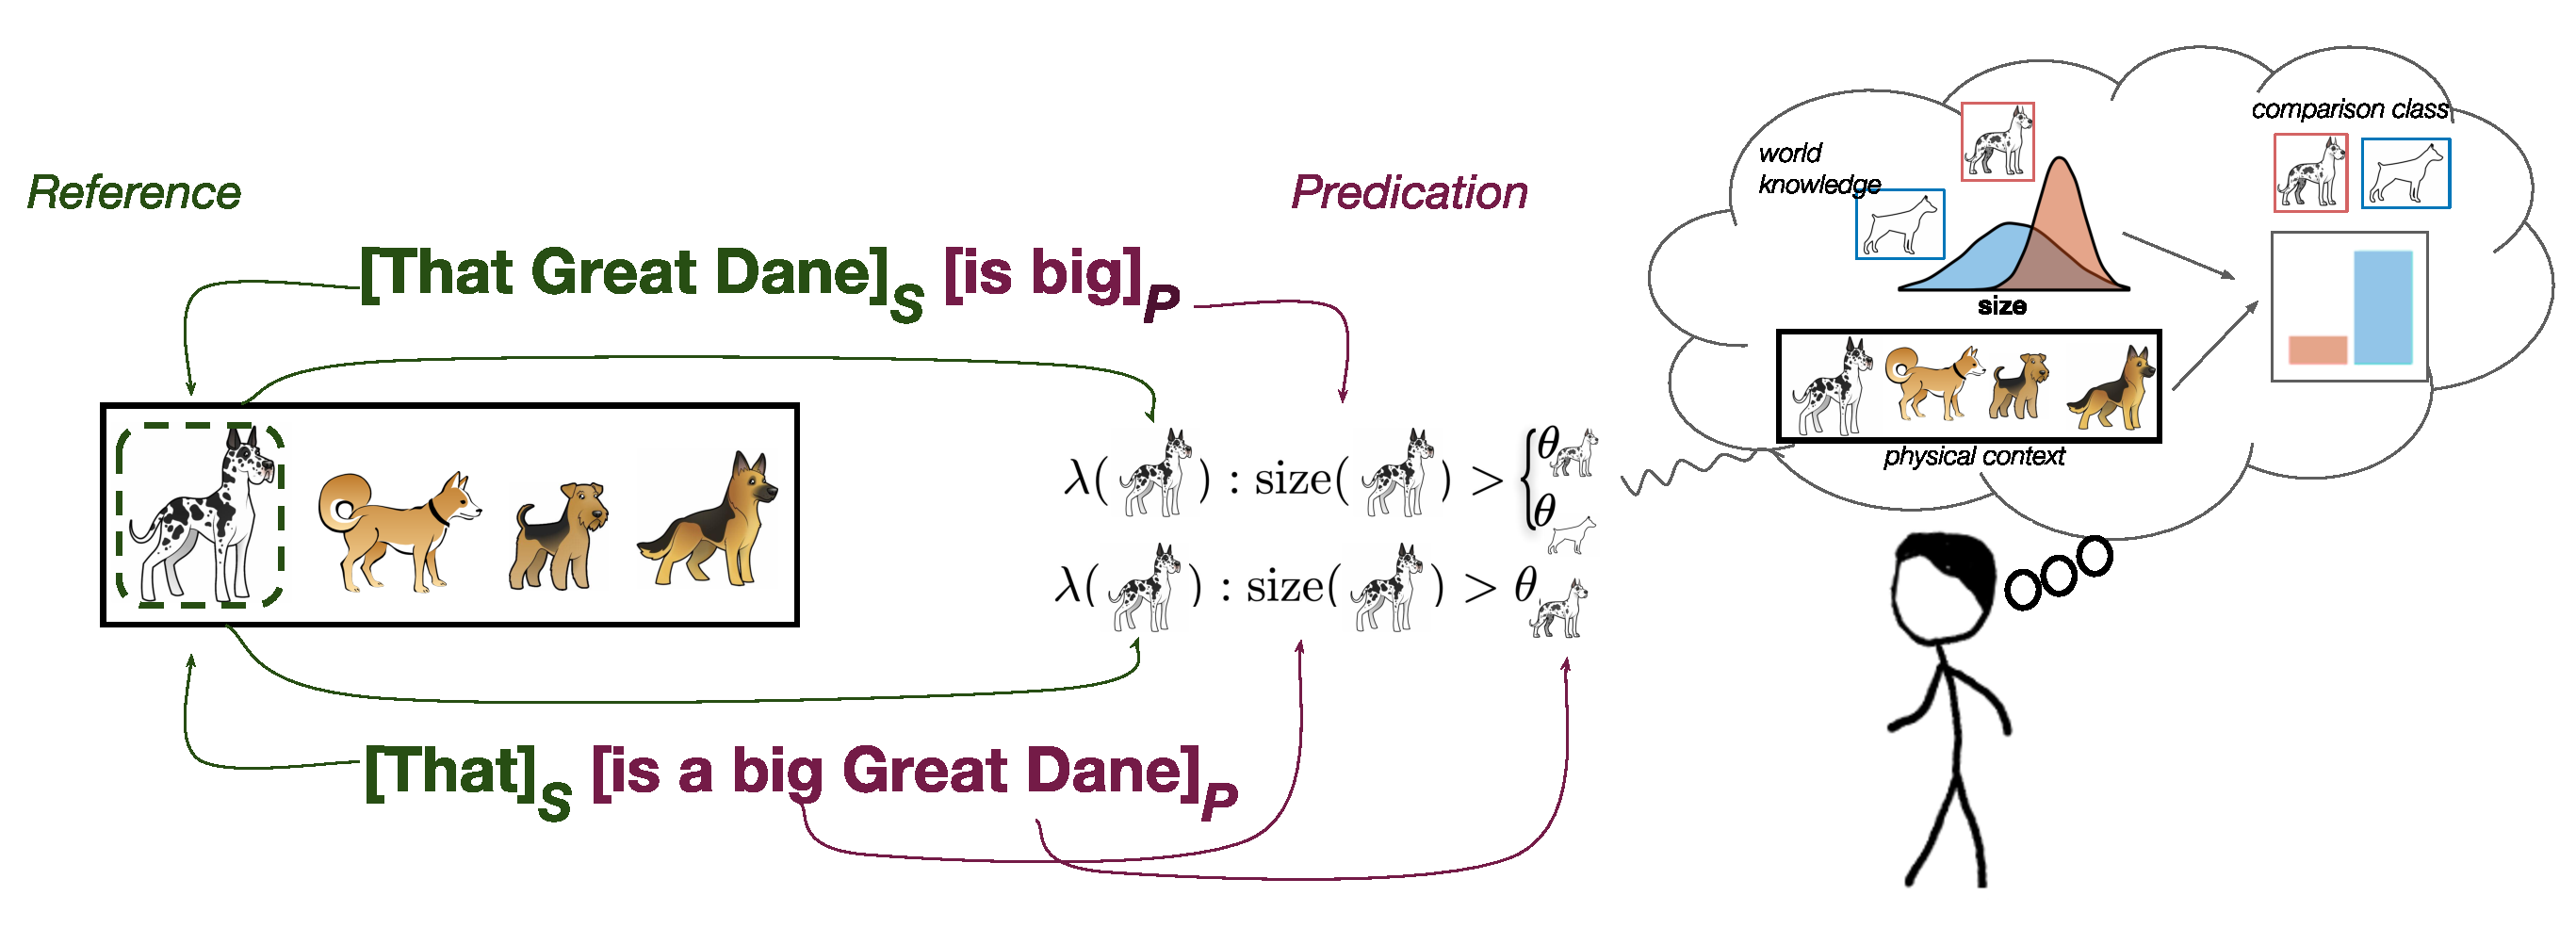
\includegraphics[width=0.9\linewidth]{ref-pred-cartoon-w-subscripts2.pdf}
\end{center}
\caption{Cartoon of the inferential account for comparison class determination. The noun (Great Dane) in a sentence can be employed either for the goal of reference (green) or predication (purple), shown in the case when this distinction is made via the syntactic position of the noun (subject S~vs.~predicate P). When the noun is used for reference (top), a listener is left with uncertainty about what to use as the comparison class (dogs or Great Danes) and integrates their world knowledge and the physical context to make this inference.  When the noun is used for predication (bottom), the listener should have less uncertainty about the comparison class: The comparison class is stipulated by the noun.}
\label{model-cartoon}
\end{figure*}

We consider the problem of comparison class inference from a functional perspective -- what goals are speakers trying to achieve when crafting their utterance, and how might these goals influence listeners’ interpretations?
In order to communicate a property of a referent, a speaker must achieve two informational goals: \emph{reference} (identifying the right target object) and \emph{predication} (ascribing a property to the referent) \cite{Reboul2001}. 
In simple sentences of the form ``\emph{Subject Predicate}'', we posit that listeners expect reference to be established by the \emph{Subject} (independent of the \emph{Predicate} asserted to hold of the subject) and that speakers aim to satisfy this expectation.\footnote{Of course, it cannot always be taken for granted that the referent is established by the subject noun (e.g., insofar as one can infer who \emph{he} is in the sentence ``He's making those outrageous tweets again.'', it is because the predicate provides a cue to the referent). We posit this relation between subject noun and reference as an expectation that listeners may hold, perhaps due to information structural reasons.
}
From this perspective, the noun in a sentence is a cue to the comparison class that is integrated with other pragmatic aspects of the utterance (Fig.~\ref{model-cartoon}):
If the noun appears in the predicate (``That’s a big Great Dane''), the speaker’s noun choice is likely non-referential, and rather a cue to the intended comparison class.  
In contrast, if the noun appears in the subject (``That Great Dane is big''), then the speaker’s choice of noun can be \emph{explained away} as intending to help the listener establish reference of the subject; the noun would then serve as a weaker cue to the comparison class and allow for other pragmatic reasoning (e.g., world knowledge and perceptual cues) to play a more substantial role in determining the comparison class \cite<e.g., the Great Dane is big for a dog;>{tessler2017warm}.


We test this reference -- predication trade-off hypothesis using a syntactic manipulation wherein the noun appears either in the subject or the predicate of a sentence involving a gradable adjective (e.g., ``That Great Dane is big''~vs.~``That's a big Great Dane''). Additionally, we test sentences where the critical noun appearing in the subject or in the predicate is always syntactically modified (e.g., ``That big sunflower is a gift'' ~vs.~``That gift is a big sunflower''), thus controlling for confounding informational cues with modification effects.
The critical test is how speakers and listeners treat these sentences in the context of a referent for whom the adjective is felicitous given one comparison class but not another (e.g., \emph{big} to describe a normal-sized Great Dane, which would be big if the comparison class is \emph{dogs} but not \emph{Great Danes}). 
We examine human judgments using three distinct dependent measures in pre-registered experiments. 


% which must be weighed in the context of other cues such as world knowledge and the physical environment. 
%We focus in particular on the question of when the noun in the sentence provides the comparison class.




%Contra a syntactic approach, the inferential hypothesis posits that the noun in a sentence is just one potential to the speaker's 
%Building on ideas for how world knowledge influences comparison class inferences \cite{tessler2017warm}, we additionally consider the role of the perceptual environment and on the influence of the noun in the sentence.

%If there exists a trade-off in the goals of reference and predication and if listeners expect speakers to establish reference in the subject of the sentence, then the influence of a speaker’s choice of noun on the comparison class will depend on  the syntactic position of the noun (subject~vs.~predicate; Fig.~\ref{model-cartoon}).




% should we include these definitions here?? (they occur in the abstract before)

%In simple, subject-predicate sentences of the form ``$S$ $P$'', where $S$ is a referential subject noun phrase and $P$ is a predicate asserted to hold of the subject, we posit that listeners expect that the referent will be made clear by the subject N -- independent of the predicate -- and that speakers aim to satisfy this expectation.
%\pt{subject NOUN PHRASE might be unclear, since we also look at sentences where the subject has no N and posit the same; we might want to add a sentence about general expectations of reference-in-subject. maybe sth like this? For simple sentences of the form "Subject Predicate", we posit that listeners expect that the referent will be made clear by the Subject - independently of the predicate, which is asserted to hold of the subject, and that speakers... }  
%We explore the implications of such a theory of 
%In this paper, we
%
%
% (e.g., the Great Dane over there by that park bench is big)
%
%We propose an inferential theory of comparison class determination: Speakers aim to achieve basic informational goals that guide how they structure their utterance, and listeners infer the most likely comparison class in light of a speaker's goals.  
%In order to successfully predicate something, one must establish reference.
%In order to successfully convey a speaker’s intended message, the $S$ $P$ sentence must clearly establish the referent of the subject NP \mht{$\leftarrow$  does this first clause already presuppose our posit that comes after (that the referent of the subject NP will be clear independently of the predicate)? i get a little confused by the phrase ``referent of the subject NP''. i feel like there is a referent, and there is a subject NP, and the subject NP is used to establish the referent in context...};
%In order to predicate something, you need to predicate of something.
%Listeners expect this to happen (the rference) in the subject... (this is an inforamtion structure point)
%If this expectation holds when interpreting gradable adjectives, 

%We examine an inferential hypothesis wherein listeners balance multiple cues to infer the comparison class. %We examine the problem from a functional perspective---what goals are speakers trying to achieve when crafting their utterance?---and focus on the role of the noun phrase (NP) in determining the comparison class (Figure \ref{model-cartoon}). %and derive novel predictions about comparison class inferences via the interaction of syntactic cues, world knowledge, and the perceptual context.
%Functionally, noun phrases (e.g., \emph{Great Dane}) can be used both for achieving the goals of \emph{reference} (i.e., getting the listener to attend the object that the speaker intends; e.g., ``Look at that Great Dane.'') and \emph{predication} (i.e., describing a property of that referent; e.g., ``This is a Great Dane.''; \cite{Reboul2001}.\footnote{The reference-predication distinction is similar to the topic--comment or given--new distinction in Information Structure \cite{lambrecht1996information}. We return to this point in the discussion.}
%When an NP appears in a sentence with a scalar adjective, the goal of predication can be understood as indicating the comparison class by communicating the speaker's perspective on the referent; a speaker using an NP to satisfy the goal of predication (e.g., via the NP appearing in the predicate of the sentence as in ``That's a big Great Dane'') can thus serve as a cue that the NP is the comparison class (i.e., \emph{it's big relative to other Great Danes}). 
%On the other hand, the presence of an NP in a sentence could also be explained by the goal of reference (e.g., by appearing in the subject of the sentence as in ``That Great Dane is big''), in which case the NP would less strongly constrain the comparison class and other pragmatic reasoning (e.g., with world knowledge) would serve to fill in the comparison class \cite<e.g., the Great Dane is big for a dog;>{tessler2017warm}.



%. However, such a purely syntactic account would stipulate that modified nouns (i.e., predicate-Ns) always set the comparison class, as well as that inferred comparison classes aren't be affected by distinct subject-Ns. Finally, if the information needed to determine the comparison class is all found in the words of the sentence, then the same sentence in a different context should not change the comparison class. 
%We note that this subject-predicate distinction could also be viewed from a syntactic-modification perspective, wherein the comparison class would be determined by the syntactically-modified N, as opposed to the unmodified N which wouldn't affect the comparison class. However, such a purely syntactic account would stipulate that modified nouns (i.e., predicate-Ns) always set the comparison class, as well as that inferred comparison classes aren't be affected by distinct subject-Ns. Finally, if the information needed to determine the comparison class is all found in the words of the sentence, then the same sentence in a different context should not change the comparison class. 


 %Across these diverse measures, we find consistent evidence for a reference-predication trade-off guiding comparison class inferences when interpreting adjectival sentences.
% Maybe use this and drop the expt. description part in intro of Experiments?

%In Experiment 1 (Syntax Rating), participants provide acceptability ratings of the syntactically-distinct sentences. In Experiment 2 (NP Production), participants produce noun phrases in different syntactic frames (e.g., ``That's a big \_\_'' vs. ``That \_\_ is big''). Finally, in Experiment 3 (Comparison Class Inference), participants paraphrase a speaker's adjectival sentence with an explicit comparison class (e.g., ``It's big relative to other \_\_''), building on the empirical paradigm of \citeA{tessler2017warm}.

%(e.g., \emph{I see this thing as a dog}) and thus should serve as a strong cue to the comparison class in case of gradable adjectives (i.e., the Great Dane is \emph{big for a Great Dane})

%to predict interpretative differences between \emph{attributive} uses of adjectives (e.g., ``That's a big Great Dane'') and \emph{predicative} uses (e.g., ``That Great Dane is big'') . 
%For attributive uses, the NP is likely to be used for predication, i.e. communicating the speaker's perspective
% conceptualization of
%on the referent (e.g., \emph{I see this thing as a Great Dane}) and thus should serve as a strong cue to the comparison class in case of gradable adjectives (i.e., the Great Dane is \emph{big for a Great Dane}). % somewhat unclear to me, see below
%In predicative uses, on the other hand, the NP is likely to be used for reference (e.g., an NP combined with a deictic such as ``That Great Dane is big''), and thus, should less strongly constrain the comparison class.
% maybe we could start with predicative adjectives because in general reference needs to be established first? And we were arguing about the attributive cases as being non-explainable in terms of reference and hence providing the CC?
%When the NP provides a weak cue to the comparison class, world knowledge can more strongly influence the comparison class \cite<e.g., the Great Dane is big for a dog;>{tessler2017warm}.
%In line with definitions of a predication act as proposed in the literature \cite{Reboul2001}, we assume that listeners always first need to establish reference before interpreting the predicate. In predicative adjective uses, the NP is considered to more likely be referential since it is combined with the deictic 'That' and constitutes a definite description. However, Donnellan proposes a distinction of definite descriptions into attributive and referential cases, where the attributive definite descriptions (non-referring) are those where the identity of the referent is unknown \cite{Reboul2001}, which supports our assumptions that the referential utility of the NP may vary. The referential vs. attributive use may be resolved pragmatically. In attributive constructions we consider, the NP is more likely to be non-referential since it is an indefinite description. NPs which do not contribute to reference are thought to "contribute bound variables and predicates" to proposition \cite{Reboul2001}. 
%We build upon the Rational Speech Act framework -  a recursive Bayesian model where the speaker and the listener coordinate an intended meaning - and suggest that listeners integrate this implicit grammatical knowledge with their world knowledge about categories and their properties and perceptual cues to infer the correct comparison class. 
% that two fundamental, informational goals of communication can serve as a basis for inferring a speaker's intended comparison class. 

\section{Experiments}
Our guiding hypothesis is that when speakers compose their utterance, the utility of a noun in reference trades-off with the utility of the noun conveying a feature value of the referent (predication) \footnote{For scalar degrees, a noun conveying a feature value amounts to setting the comparison class of the respective gradable adjective}; utility in reference can then \emph{explain away} the utility of using a noun to set the comparison class. 
We operationalize utility in reference via the syntactic frame in which the noun phrase appears: if the noun appears in the subject of the sentence (That NOUN is ADJ), it is likely to be used for reference and less likely to set the comparison class. If the noun appears in the predicate of the sentence (That's an ADJ NOUN), it is unlikely to be used for reference and more likely to set the comparison class. 

In all of our experiments, we use the ADJs \emph{big} and \emph{small} because of the simplicity with which the feature value (i.e., size) can be conveyed through visual presentation and because they convey a salient feature about which participants likely have strong expectations for different categories (e.g., Great Danes are generally big dogs; goldfish are generally small fish; etc.). 
Referents were always described using the size adjective consistent with these general expectations (e.g., \emph{Great Dane -- big}, \emph{goldfish -- small}), to allow for the possibility of either subordinate (Great Dane) or basic-level (dog) comparison classes.
%Thus, given world knowledge, both the subordinate-level or basic-level comparison class could be felicitous.%, though the basic-level is more likely \textit{a priori} (i.e., the Great Dane is likely to be \textit{big for a dog}, but could also be \textit{big for a Great Dane}).
The preregistrations and full experimental procedures can be viewed at \url{tinyurl.com/rcsyz9f}.\footnote{All data and code can be found under \url{https://github.com/polina-tsvilodub/refpred}}

%; thus, referential utility can serve as a cue to the comparison class for listeners and a guide for speaker preferences about  . %
%  which we examine using the subject vs. predicate contrast in where the NP appears. 


%In Experiment 1 (Syntax Rating), participants provide acceptability ratings of the syntactically-distinct adjectival sentences to describe an object for which the size adjective would be felicitous given one comparison class but not another. In Experiment 2 (NP Production), tests if participants produce different nouns given different syntactic frames (e.g., ``That's a big \_\_'' vs. ``That \_\_ is big''). Finally, Experiment 3 (Comparison Class Inference) investigates listeners' comparison class inferences as driven by the syntax, the noun phrase, and the immediate perceptual context in which the sentence is uttered, via participants paraphrasing a speaker's adjectival sentence with an explicit comparison class (e.g., ``It's big relative to other \_\_''), building on the empirical paradigm of \citeA{tessler2017warm}.
%Experiment 1 tests if participants prefer one noun position in the sentence over the other to describe an object for which the size adjective \emph{big} would be felicitous given one comparison class but not another. Experiment 2 tests if speakers produce different nouns in different syntactic frames to describe the same object. Finally, Experiment 3 investigates listeners' comparison class inferences as driven by the syntax, the noun phrase, and the immediate perceptual context in which the sentence is uttered.

\begin{figure*}[t]
\begin{center}
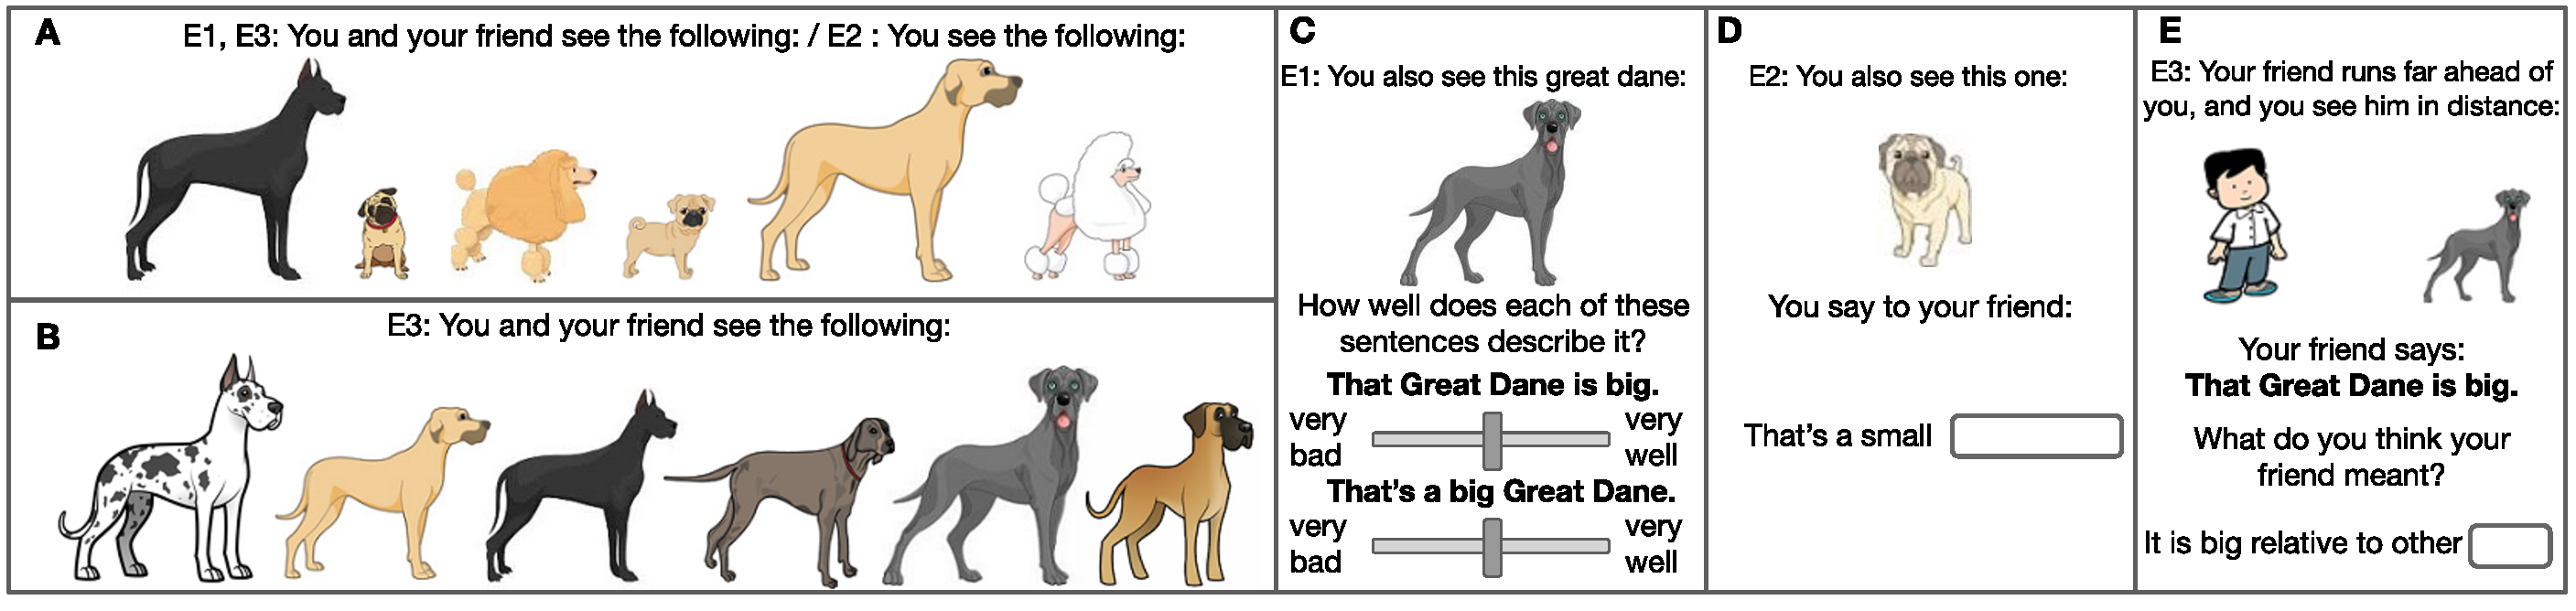
\includegraphics[width=\textwidth]{screenshots.pdf}
\end{center}
\caption{Overview of Experiments 1-3. A - B: Example context stimuli. A: Basic-level contexts used in Expts.~1-3. B: Subordinate context from Expt.~3. C - E: Example test questions with referents. C: Syntax Rating trial (Expt.~1) with a referent from a large-subordinate category referred to with a subordinate-level noun. D: Noun free-production trial (Expt.~2) with a referent from a small-subordinate category described with a predicate-noun syntactic frame. E: Comparison Class Inference trial (Expt.~3) with a referent from a large-subordinate category described with a subject-noun syntactic frame using a subordinate-level noun.} 
\label{screenshots}
\end{figure*}
\begin{table}[t]
\small{
\begin{center}
\caption{Experimental items: each basic-level context had two potential targets from an either saliently small or saliently big subordinate category within the basic-level class. Items marked with * were used in Expt. 2.}
\label{tab:stimuli}
\vskip 0.12in
\fontsize{10}{11}\selectfont
\begin{tabularx}{\linewidth}{lll}
\hline
 Basic-level category & Smaller referent & Bigger referent\\
\hline
 Dogs & Pug & Great Dane \\
 Dogs & Chihuahua & Doberman\\
 Birds & Hummingbird & Eagle  \\
 Fish & Goldfish & Swordfish \\
 Flowers & Dandelion & Sunflower\\
 Trees & Bonsai & Redwood\\
Birds* & Sparrow* & Goose* \\
Birds* & Canary* & Swan* \\
Fish* & Clownfish* & Tuna* \\
Flowers* & Daisy* & Peony* \\
\hline     
\end{tabularx}
\end{center}
}
\end{table}

\subsection{Experiment 1: Syntax rating} In this experiment, participants rated how well each of two sentences differing in the position of the noun described the target. The noun was either the basic-level (e.g., dog) or the subordinate target label (e.g., Great Dane; within-subjects).



\subsubsection{Participants} We recruited \rlgetvariable{myvars-rating.csv}{nSubj} participants from Amazon's Mechanical Turk; participants in all experiments were restricted to those with US IP addresses and at least a 95\% work approval rating. We excluded \rlgetvariable{myvars-rating.csv}{nExcludedTotal} for reporting a native language other than English, failing a comprehension check or providing the same responses on every trial. The experiment took about 5 minutes and participants were compensated \$0.80. %\rlgetvariable{myvars-rating.csv}{nFailedWarmUp}  and \rlgetvariable{myvars-rating.csv}{nFailedMains} for  


\subsubsection{Materials} 
All experiments used the same materials. 
%We used the positive- and negative-form gradable adjectives describing size: \emph{big} and \emph{small}. %In all experiments, the critical sentence(s) with the gradable adjective describe a target object presented visually alongside other objects (the \emph{visual context}; Figure~\ref{screenshots}A,B).
Nouns and referent pictures were chosen from five \emph{basic-level categories} in the animal and plant domains: dogs, birds, fish, flowers, trees.
Within each basic-level category, we chose target objects from \emph{subordinate level categories} about which people have prior expectations concerning the size of members of those categories (Table \ref{tab:stimuli}).
%For example, Great Danes are generally big relative to other dogs; goldfish are generally small relative to other fish. 
%Targets are described using the size adjectives consistent with these general expectations (e.g., \emph{Great Dane -- big}, \emph{goldfish -- small}).
%Thus, given world knowledge, both the subordinate-level or basic-level comparison class could be felicitous.%, though the basic-level is more likely \textit{a priori} (i.e., the Great Dane is likely to be \textit{big for a dog}, but could also be \textit{big for a Great Dane}).

\subsubsection{Procedure}
Participants completed two comprehension check trials and six main trials. In the comprehension check trials, participants saw a picture (e.g., a purple chair), read pairs of sentences describing it (e.g., ``The chair is blue'' and ``The chair is yellow''), and were asked to rate on a slider how well each of the sentences described the referent.

In the main trials, participants read: ``You and your friend see the following:'' above a context picture with other members of the same basic-level category (e.g., a group of dogs; Figure~\ref{screenshots}A). 
Six different basic-level contexts were created from the five categories depicting groups of several members belonging to different subordinate categories (e.g., dogs of different breeds, including the target and filler subordinate categories, such as Great Danes, pugs and poodles; Table~\ref{tab:stimuli}).
Below the context they read ``You also see this \emph{subordinate label}'' and saw the referent pictured.
% possibly cut the following paragraph?
%The visual size of the picture of the referent is manipulated such that it appears incongruent with the general expectations of that subordinate category (i.e., a Great Dane, which we would expect to be large, is actually small relative to other Great Danes in the context; Fig~\ref{screenshots}C compared to context in Fig.~\ref{screenshots}A). 
%This subtle visual disparity was imposed in order to enhance the difference in felicity between the adjective used with a basic-level~vs.~subordinate level comparison class (e.g., the Great Dane is \emph{big for a dog} but probably not \emph{big for a Great Dane}).

Participants rated how well two sentences described the target, using sliders ranging from \textit{very bad} to \textit{very well}. The sentences differed in whether the noun N appeared in the subject or predicate of the sentence (e.g., Predicate N: ``That's a big Great Dane''; Subject N: ``That Great Dane is big''; Fig.~\ref{screenshots}C), and the order in which the sentences and corresponding sliders appeared on the page was randomized between-subjects. 
Trials differed in whether the noun was the subordinate referent label (e.g., \emph{Great Dane}) or the basic-level label (e.g., \emph{dog}), in randomized order. 
Each participant saw only one of the two possible targets for each context (e.g., either the Great Dane or the pug for the dog basic-level context).


\subsubsection{Results} 
We found no effect of the slider presentation order (syntactic conditions), so the data was collapsed across the two conditions for all analyses. 
%shows the mean ratings provided for subordinate and basic-level NPs in the subject and predicate-NP syntactic frames.
Consistent with our prediction,  participants substantially dispreferred sentences with the subordinate noun in predicate position compared to the subject position (Figure~\ref{syntax-rating}), confirmed by a Bayesian generalized linear mixed-effects model with main effects of syntax, the noun phrase, and their interaction, as well as a maximal random effects structure.\footnote{In lmer-style syntax: \texttt{rating $\sim$ syntax * NP + (1 + syntax*NP | subject) + (1 + syntax*NP | target)}}
We found an interaction between the syntax and the noun-label  (mean and 95\% Bayesian credible interval: $\beta = \rlgetnum{expt1_brm.csv}{Rowname}{syntax:NP}{Estimate}{2}  [\rlgetnum{expt1_brm.csv}{Rowname}{syntax:NP}{l.95..CI}{2}, \rlgetnum{expt1_brm.csv}{Rowname}{syntax:NP}{u.95..CI}{2}]$), as well as an overall preference for the basic-level nouns ($\beta = \rlgetnum{expt1_brm.csv}{Rowname}{NP}{Estimate}{2} [\rlgetnum{expt1_brm.csv}{Rowname}{NP}{l.95..CI}{2},\rlgetnum{expt1_brm.csv}{Rowname}{NP}{u.95..CI}{2}] $) and subject-N syntax ($\beta = \rlgetnum{expt1_brm.csv}{Rowname}{syntax}{Estimate}{2} [\rlgetnum{expt1_brm.csv}{Rowname}{syntax}{l.95..CI}{2}, \rlgetnum{expt1_brm.csv}{Rowname}{syntax}{u.95..CI}{2}] $). 
In exploratory analyses, we
% found no effects of the target size (Great Dane ~vs.~ pug). We 
observed considerable variation in the by-target intercepts (e.g., \emph{sunflower} item received overall lower ratings), probably due to a varying basic-level label bias of the single items (the subordinate labels were more salient for some items than for others; $\beta = \rlgetnum{expt1_random_brm.csv}{Rowname}{sd(Intercept)}{item.Estimate}{2} [\rlgetnum{expt1_random_brm.csv}{Rowname}{sd(Intercept)}{item.l.95..CI}{2}, \rlgetnum{expt1_random_brm.csv}{Rowname}{sd(Intercept)}{item.u.95..CI}{2}]$). 
% I did an lmer analysis with size effect, the main effect was p=0.047, the syntax-NP-size interaction p=0.021
%Participants discriminate the felicity of sentences involving the same NPs and same adjectives, depending on the syntactic position of the NP. 
%This result is consistent with the hypothesis that the syntactic position of the NP modulates the strength of the cue that the NP provides towards the comparison class. 

\subsection{Experiment 2: Free-production of noun}
If the syntactic position of the noun modulates the strength of the cue the noun provides towards the comparison class, we would also expect speakers to produce different nouns depending on the noun's syntactic position, which we test here.

\subsubsection{Participants}
We recruited \rlgetvariable{myvars-np.csv}{nSubj} participants and excluded \rlgetvariable{myvars-np.csv}{nExcludedTotal} for implementation glitches, non-native English language, or failing warm-up trials more than 4 times. The experiment took about 7 min and participants were compensated \$1.00. %\rlgetvariable{myvars-np.csv}{nNonEN} for  and \rlgetvariable{myvars-np.csv}{nFailedWarmUp} for  

\begin{figure}[t]
\begin{center}
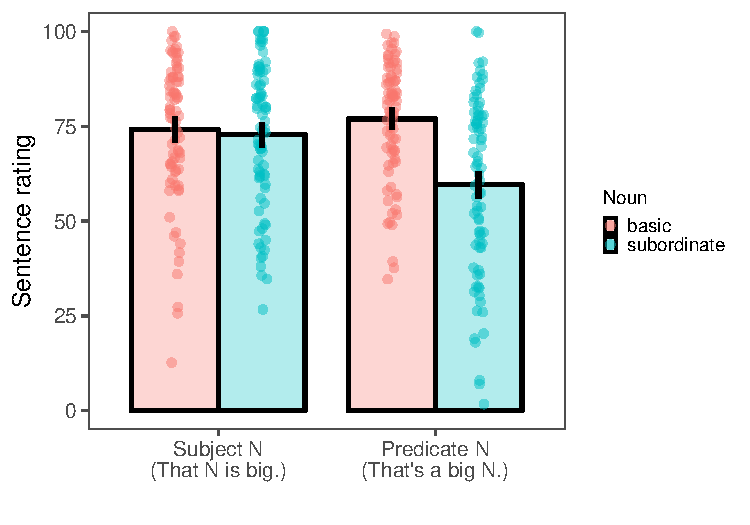
\includegraphics[width=\linewidth]{expt-syntax-rating-prereg-bars-revised.pdf}
\end{center}
\vspace{-0.3cm}
\caption{Experiment 1 mean ratings for how well sentences which differed in the syntactic position of the noun (x-axis)  and the noun-label (color) described the referent, a typically-sized member of the subordinate category (e.g., a normal-sized Great Dane).  Points represent participant means within condition. Error-bars denote bootstrapped 95\% confidence intervals (bootstrapping independent of random-effects structure).
%\vspace{-0.5cm}
}
\label{syntax-rating}
\end{figure}

%\vspace{-1.5cm}
\subsubsection{Procedure}
The main trials were divided into two blocks, and before each block, participants completed warm-up trials. The warm-up trials were designed to elicit category labels at different levels of abstraction (e.g., ``Great Dane'', ``pug'', ``dog'') by filling-in labeling sentences, for which they were provided corrective feedback. %Two sentences appeared below each target reading ``This is a \_\_'', and one sentence appeared at the bottom of the page reading ``These are both \_\_.''
%Participants supplied an incorrect label, they were provided the correct label and were required to correct their response before proceeding.
The same subordinate referents were used as targets in the main trials. 
Trial order within each warm-up and main block was randomized. We used the same contexts as in Experiment 1 and created four additional basic-level contexts (Table \ref{tab:stimuli}). 
Six contexts were randomly sampled for each participant (three per block). 

On the main trials, subjects saw “You see the following:” above the context picture (as in Expt.~1; Fig~\ref{screenshots}A). Below, they read “You also see this one:” and saw the picture of the referent (e.g., a Great Dane or a pug). They were told “You say to your friend:”, followed by either a subject-N or predicate-N sentence frame (between-subjects), where the noun was omitted (e.g., “That \_\_ is big“~vs.~“That’s a big \_\_ ''; Fig.~\ref{screenshots}D). Each participant saw only either the big or the small target for each basic-level category. 
The free-production responses were categorized by hand into subordinate or basic-level labels of the referent. 16 uncategorizable responses (1.4\%) were excluded from the analysis.
\begin{figure}[t]
\begin{center}
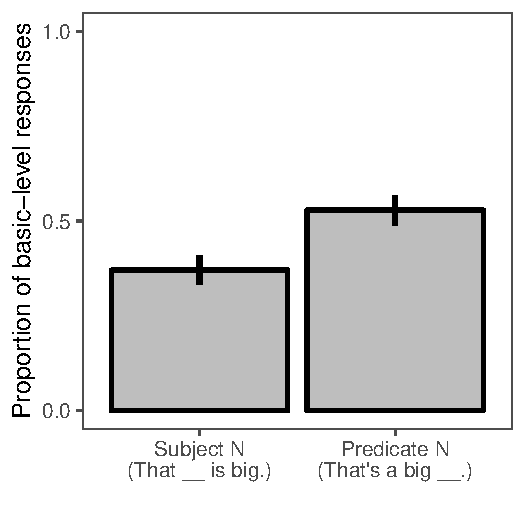
\includegraphics[width=0.7\linewidth]{expt-np-prod-prereg-bars-revised.pdf}
\end{center}
\vspace{-0.3cm}
\caption{Experiment 2: Proportions of freely-produced basic-level labels (e.g., \emph{dog}) in different syntactic frames (x-axis) when the referent was a typically-sized member of a subordinate category (e.g., a normal-sized Great Dane). Error-bars denote 95\% bootstrapped confidence intervals.}
\vspace{-0.3cm}
\label{np-production}
%\vspace{-0.2cm}
\end{figure}
\subsubsection{Results}
Participants produced basic-level nouns at a higher rate in the predicate than in the subject position (Figure \ref{np-production}), confirmed by a logistic Bayesian mixed-effects regression model, predicting the response category (basic-level vs. subordinate) by an intercept, the main effect of syntax %(contrast coded, subject vs. predicate NP) 
and by-participant and by-referent random intercepts and a by-referent random slope effect of syntax.\footnote{In lmer syntax: \texttt{response\_category $\sim$ syntax + (1 | subject) + (1 + syntax | target)}} Participants were appreciably more likely to use basic-level labels in the predicate position ($\beta = \rlgetnum{expt2_brm.csv}{Rowname}{syntax_contr}{Estimate}{2} [\rlgetnum{expt2_brm.csv}{Rowname}{syntax_contr}{l.95..CI}{2}, \rlgetnum{expt2_brm.csv}{Rowname}{syntax_contr}{u.95..CI}{2}]$). 
%In exploratory analyses, we did not find effects of target size (e.g., Great Dane vs. pug). 
%Similar to Expt.~1, exploratory analyses show considerable by-target variation in terms of the random intercept ($\beta = \rlgetnum{expt2_random_brm2.csv}{Rowname}{Intercept}{target.Estimate}{2} [\rlgetnum{expt2_random_brm2.csv}{Rowname}{Intercept}{target.l.95..CI}{2}, \rlgetnum{expt2_random_brm2.csv}{Rowname}{Intercept}{target.u.95..CI}{2}] $), likely due to differing subordinate-label accessibility (e.g., \emph{swan} is more accessible than \emph{peony}). Within the predicate noun trials, small targets elicited significantly more basic-level labels than big targets (e.g., pug $\rightarrow$ \emph{small dog} more so than Great Dane $\rightarrow$ \emph{big dog}; $\beta = \rlgetnum{expt2_predicate_brm.csv}{Rowname}{size_contr}{Estimate}{2} [\rlgetnum{expt2_predicate_brm.csv}{Rowname}{size_contr}{l.95..CI}{2}, \rlgetnum{expt2_predicate_brm.csv}{Rowname}{size_contr}{u.95..CI}{2}]$). % when subsetting the data by syntax, the re is a size effect in the predicate condition (beta = 1.61 [0.26, 3.21]).    
%Participants are more likely to choose the NP corresponding to the felicitous comparison class in the predicate syntactic frame. %produce an NP corresponding to the more felicitous -- basic-level -- comparison class in the predicate syntactic frame.
\subsection{Experiment 3: Comparison class inference}% In this experiment we elicited comparison classes inferred by listeners given different visual contexts, noun, and syntactic frames of the critical utterance (within-subjects). 
According to our inferential account, comparison class inferences should be driven by the noun (\emph{dog} or \emph{Great Dane}) to the extent that the usage of the noun cannot be explained away as achieving the goal of reference.
Our first two experiments support this view: Participants dispreferred sentences like ``That's a big Great Dane'' when the subordinate comparison class was infelicitous for the referent (i.e., the Great Dane was not big for a Great Dane).
In this experiment, we provide a more direct test of our account by explicitly measuring comparison class inferences.

Our experimental design manipulates three factors within-subject: syntactic position of the noun, level-of-abstractness of the noun (basic-level vs. subordinate-level vs. underspecified; e.g., \emph{dog} vs. \emph{Great Dane} vs. \emph{one}), and visual context (e.g., other dogs vs. other Great Danes).
%The inferential account provides a natural avenue for visual context to influence comparison class inferences.
Foremost, the inferential account provides a natural avenue for visual context to influence comparison class inferences: The noun in the sentence may not provide the comparison class if the visual context is very salient. 
Second, when the noun's usage can be explained away by its utility in reference, comparison class inferences should be more strongly driven by world knowledge (e.g., Great Danes are big dogs) or the visual context. 
%By contrast, a purely syntactic-based account would predict no effect of visual context. %: If the information needed to determine the comparison class is all found in the words of the sentence, then the same sentence in a different context should not change the comparison class. 
We include an underspecified noun condition using the anaphoric ``one'' to provide a base-line measure of the influence of visual context on comparison class inferences: In a context with varying types (basic-level context; Fig.~\ref{screenshots}A), anaphoric ``one'' should be interpreted as ``dog''; when the context provides animals of the same type (subordinate-level context; Fig.~\ref{screenshots}B), anaphoric ``one'' is more likely to be interpreted more narrowly \cite<``Great Dane'';>{goldberg2017one}.
%When the noun does contribute to the goal of reference, we predict comparison class inferences should be driven by the visual context.

\subsubsection{Participants} 

We recruited \rlgetvariable{myvars-infer.csv}{nSubj} participants and excluded \rlgetvariable{myvars-infer.csv}{nExcludedTotal} for either reporting other native languages than English, failing a task comprehension check, or failing warm-up trials more than 4 times after feedback. The experiment took about 9 minutes and participants were compensated \$1.20. % \rlgetvariable{myvars-infer.csv}{nFailedCCWarmUp} for d \rlgetvariable{myvars-infer.csv}{nFailedWarmUp} for  

\subsubsection{Procedure} Before the main trials, participants completed a comparison class paraphrase of the kind used in the main trials, for which they were provided corrective feedback.
%: they rephrased what they understand a speaker to mean by using an explicit comparison class. Participants read that a speaker said ``The Empire State Building is tall'' and were asked what the speaker meant: ``The Empire State Building is tall relative to other \_\_''. 
%Participants had to correct their response if they provided an infelicitous comparison class. %(viable responses included: buildings, skyscrapers, constructions, houses).
Following this comprehension test, participants completed two blocks of warm-up and main trials, akin to  Expt.~2.

In the main trials, participants read ``You and your friend see the following:" above a context picture of either subordinate-level or basic-level distractors (Fig.~\ref{screenshots}A, B). 
Below the context picture, they read ``Your friend runs far ahead of you, and you see him in the distance'' with a cartoon person standing next to the referent (e.g., a Great Dane) in the distance so that the referent size could not serve as a cue to the comparison class (Fig.~\ref{screenshots}E). 
Participants read ``Your friend says: [critical sentence]", which could vary by both syntactic position of the noun and the noun-label's level-of-abstractness (e.g., ``That Great Dane is big'', ``That's a big dog'', ``That one is big'', etc.). 
%The noun could be the subordinate target label (e.g., Great Dane), basic level label (dog), or the underspecified anaphoric \emph{one} (e.g., ``That one is big''). 
%We used \emph{one} in order to measure the baseline effect of visual context on comparison class inferences. %and to test whether listeners infer the comparison class from visual context and world knowledge (i.e. that the basic-level comparison class is a priori more likely to be felicitous) if the NP does not provide informative cues towards the comparison class. Therefore, we expected the comparison class to be the basic-level category of the referent given basic-level context (e.g. dogs) and the subordinate category given the subordinate context (e. g. great danes), though we expected to possibly see a basic-level bias, such that “dogs” was the a priori preferred comparison class..
Participants were asked: ``What do you think your friend meant?" and responded in the sentence frame: ``It is big (small) relative to other \_\_” (Fig.~\ref{screenshots}E).
Participants completed 12 trials which could vary by syntactic frame [subject vs. predicate], visual context [subordinate vs. basic], and noun [subordinate vs. basic vs. \emph{one}].\footnote{Due to a coding error, condition balancing occurred at the level of individual factors independently but not jointly (i.e., participants did not complete all 12 unique trial types, but did complete equal numbers of each level of each factor).}
%\pt{this is not completely correct since i messed up the randomization..}.

%Our design attempts to constrain the sources of information that could be used for the comparison class inference. 
%In particular, we wanted to remove the actual size of the referent as a potential source of information. 
%Thus, we intentionally presented the friend/speaker as ``far ahead of you'' so that the size of the friend would not be a cue to the size of the referent, which could be used to determine the comparison class. 

%with the constraint that both small and big referents of a basic-level category (e.g., Great Danes and pugs) appeared in the same block, with one appearing in the basic-level visual context and the other appearing in its subordinate-level visual context (e.g., Great Dane appears with other dogs and the pug appears with other pugs). 

%\subsubsection{Predictions} %We predict comparison class inferences as a result of multiple cues operating in distinct manners. %This should be modulated by the syntactic position of the NP, with %In the abstract, comparison class inferences should be driven a basic-level bias \cite{rosch1975} %We predict referential utility of an NP should influence comparison class inferences. %In the basic-level visual context, we expected the subordinate NP to signal a subordinate comparison class more strongly when it appeared in predicate position than in the subject; we use the underspecified-NP (``one'') as the baseline comparison.  %In a subordinate visual context, the subordinate NP did not restrict the comparison class more beyond the context if the visual context pushed the basic-level category to floor, so the inferred comparison classes should correspond to baseline; if, however, the baseline comparison class inferences for the basic-level category were not at floor with the subordinate visual context, we expected the predicate syntax with the subordinate NP to further restrict the comparison class to the subordinate category. Similarly, the basic-level NP in the basic-level context did not restrict the comparison class more than the context, such that should be no differences in the basic-level inference proportions compared to the baseline (inferences drawn from ‘one’). In the subordinate context, however, the basic-level NP provided a more general comparison class than the context, such that the basic-level inference proportion should be higher given the predicate NP than the baseline; there might be no difference between the predicate and the subject basic-level NP since the subject NP cannot be explained by the goal of reference - its referential utility is low (all the distractors are dogs) and hence the NP was explained by predication - communicating the comparison class. %In the main trials, participants saw both possible subordinate targets within a basic-level category (e.g. both a great dane and a pug for dogs) (Table \ref{tab:stimuli}). \mht{<-- is this different from the other experiments?} %The type of context was randomly sampled, resulting in six main trials with basic-level contexts and six main trials with subordinate contexts per participant.
\begin{figure}[t]
	\begin{center}
		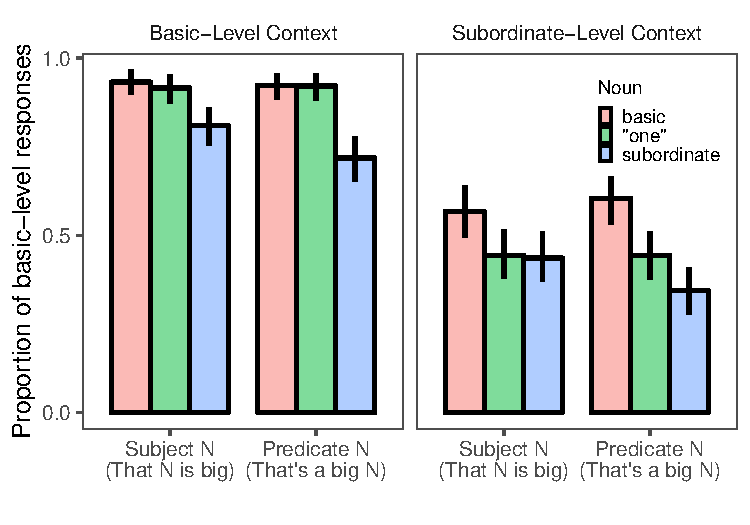
\includegraphics[width=\linewidth]{expt3-cc-inference-revised.pdf}
	\end{center}
	\vspace{-0.5cm}
	\caption{Experiment 3 results. Proportions of inferred comparison classes in terms of basic-level responses (e.g.,~“...big relative to other dogs”) as a function of syntactic position of the noun (x-axis), noun-label (color), and context (facets).
	Context strongly modulated the comparison class (left~vs.~right panel). 
	The noun additionally provided a cue to the comparison class (red~vs.~blue) bars, even in subject position. 
	The effect of noun (red~vs.~blue) is modulated by syntax. 
	Error-bars denote bootstrapped 95\% confidence intervals.
	}
	\vspace{-0.3cm}
	\label{cc-inference}
\end{figure}

\subsubsection{Results} 
Responses were categorized by hand as either basic-level or subordinate labels. 
Six of participants' responses were superordinate category labels (e.g., ``animals''), which we collapsed with the basic-level responses. 
39 uncategorizable responses (1.6\%) were excluded from the analysis. 

To test our predictions, we constructed a Bayesian logistic mixed-effects regression model that predicted the response category (basic-~vs.~subordinate-level comparison class) from the syntax, context, noun-label and the pair-wise two-way and three-way interactions, with a maximal random effects structure afforded by our design \cite{barr2013}.\footnote{ \texttt{response\_category $\sim$ syntax*NP*context + (1 + syntax + NP + context || subject) + (1 + syntax*NP*context || target)}. We set the correlation of random effects to be 0, for computational tractability.}
A simple, syntactic account of comparison class determination would hold that the noun in the sentence determines the comparison class: the same sentence should receive the same comparison class regardless of context.
Contra this account, we observe a large main effect of context: given the exact same sentence, more basic-level comparison classes were inferred overall from the basic- than subordinate-level context  ($\beta = \rlgetnum{expt3_full_brm_revised2.csv}{Rowname}{context_sum}{Estimate}{2} [\rlgetnum{expt3_full_brm_revised2.csv}{Rowname}{context_sum}{l.95..CI}{2},  \rlgetnum{expt3_full_brm_revised2.csv}{Rowname}{context_sum}{u.95..CI}{2}]$; Fig.~\ref{cc-inference}, left~vs.~right facets) and in particular, for our baseline anaphoric \emph{one} condition ($\beta = \rlgetnum{expt3_3way_full_contrasts_wProbs.csv}{Rowname}{context_one_v_mean}{mean}{2} [\rlgetnum{expt3_3way_full_contrasts_wProbs.csv}{Rowname}{context_one_v_mean}{X.95.}{2}, \rlgetnum{expt3_3way_full_contrasts_wProbs.csv}{Rowname}{context_one_v_mean}{u95.}{2}]$).
We additionally observe a main effect of noun-label regardless of the syntactic position of the noun, arguing against an account wherein only syntactically-modified nouns (``ADJ NOUN'') provide the comparison class: basic-level nouns were overall more likely to trigger basic-level comparison classes compared to subordinate nouns ($\beta = \rlgetnum{expt3_3way_full_contrasts_wProbs.csv}{Rowname}{basic_v_sub}{mean}{2} [\rlgetnum{expt3_3way_full_contrasts_wProbs.csv}{Rowname}{basic_v_sub}{X.95.}{2}, \rlgetnum{expt3_3way_full_contrasts_wProbs.csv}{Rowname}{basic_v_sub}{u95.}{2}$]).
These noun-labels influenced comparison classes above and beyond the baseline for the perceptual contexts, as indexed by the anaphoric \emph{one} condition: basic~vs.~\emph{one} ($\beta = \rlgetnum{expt3_3way_full_contrasts_wProbs.csv}{Rowname}{basic_v_one}{mean}{2} [\rlgetnum{expt3_3way_full_contrasts_wProbs.csv}{Rowname}{basic_v_one}{X.95.}{2}, \rlgetnum{expt3_3way_full_contrasts_wProbs.csv}{Rowname}{basic_v_one}{u95.}{2}]$) and subordinate~vs.~\emph{one} ($\beta = \rlgetnum{expt3_3way_full_contrasts_wProbs.csv}{Rowname}{sub_v_one}{mean}{2} [\rlgetnum{expt3_3way_full_contrasts_wProbs.csv}{Rowname}{sub_v_one}{X.95.}{2}, \rlgetnum{expt3_3way_full_contrasts_wProbs.csv}{Rowname}{sub_v_one}{u95.}{2}]$). 
%($\beta = 1.23 [0.3, 2.2]$) and subordinate-level labels receiving fewer basic-level comparison classes than \emph{one} ($\beta = -1.57 [-0.6, -2.6]$). \mht{replace with numbers read in from .csv... also, add basic vs. sub contrast}.
We also observe that a subordinate noun can be the minority comparison class response even when the noun is syntactically modified by the adjective (e.g., ``big Great Dane'' $\rightarrow$ for a dog; Fig.~\ref{cc-inference}, left-facet, blue-bar). %\pt{should we mention 'one'specifically once more?}



%In addition to a global preference for basic-level comparison classes ($\beta = \rlgetnum{expt3_brm.csv}{Rowname}{Intercept}{Estimate}{2} [\rlgetnum{expt3_brm.csv}{Rowname}{Intercept}{l.95..CI}{2},  \rlgetnum{expt3_brm.csv}{Rowname}{Intercept}{u.95..CI}{2}]$), 

%We see that the basic noun vs. subordinate noun difference was maintained even in the subject position (Fig.~\ref{cc-inference}; red~vs.~blue bars), consistent with the inferential account in which the choice of noun is a cue to a speaker's conceptualization of the referent.

We find evidence in support of the Noun (basic~vs.~sub) x Syntax interaction predicted by the reference -- predication trade-off hypothesis: Participants provided more subordinate-level comparison classes when the subordinate-level noun appeared in the predicate than when it appeared in the subject, in comparison to the basic-level noun (red~vs.~blue bars X x-axis; $\beta = \rlgetnum{expt3_3way_full_contrasts_wProbs.csv}{Rowname}{syntax_basic_v_sub}{mean}{2} [\rlgetnum{expt3_3way_full_contrasts_wProbs.csv}{Rowname}{syntax_basic_v_sub}{X.95.}{2}, \rlgetnum{expt3_3way_full_contrasts_wProbs.csv}{Rowname}{syntax_basic_v_sub}{u95.}{2}]$).
%We observe suggestive evidence in support of the Noun (basic~vs.~sub) x Syntax interaction predicted by the reference -- predication trade-off hypothesis (Fig.~\ref{cc-inference}; red~vs.~blue bars vs. x-axis; 98\% of the posterior distribution of the interaction was greater than 0, analogous to a one-tailed test; $\beta = \rlgetnum{expt3_3way_full_contrasts_revised2.csv}{Rowname}{syntax_basic_v_sub}{mean}{2} [\rlgetnum{expt3_3way_full_contrasts_revised2.csv}{Rowname}{syntax_basic_v_sub}{X.95.}{2}, \rlgetnum{expt3_3way_full_contrasts_revised2.csv}{Rowname}{syntax_basic_v_sub}{X95..}{2}]$). To further explore the Noun x Syntax interaction, we built a regression model that assumed only a fixed-effect of context \footnote{\texttt{response\_category $\sim$ syntax*N + context + (1 + syntax + N + context || subject) + (1 + syntax + N + context || item) }} and confirmed the N (basic~vs.~sub) x Syntax interaction ($\beta = \rlgetnum{expt3_2way_full_contrasts_revised2.csv}{Rowname}{syntax_basic_v_sub}{mean}{2} [\rlgetnum{expt3_2way_full_contrasts_revised2.csv}{Rowname}{syntax_basic_v_sub}{X.95.}{2}, \rlgetnum{expt3_2way_full_contrasts_revised2.csv}{Rowname}{syntax_basic_v_sub}{X95..}{2}]$). %($\beta = -0.49 [-0.86, -0.05]$).
We further examine the syntax X noun interaction in the context of the N~vs.~\emph{one} contrasts and find suggestive evidence that this interaction is driven by the subordinate noun.%, consistent with the reference -- predication trade-off hypothesis because the subordinate-noun is referentially informative  in our paradigm (as opposed to the basic-level noun, which is never referentially informative).
Specifically, we find a $\rlgetnum{expt3_3way_full_contrasts_wProbs.csv}{Rowname}{syntax_sub_v_one}{prob_lt_0}{1}$\% probability that the subordinate-N~vs.~\emph{one} x Syntax interaction term was less than 0 (i.e., more subordinate comparison classes when the noun was in the predicate; $\beta = \rlgetnum{expt3_3way_full_contrasts_wProbs.csv}{Rowname}{syntax_sub_v_one}{mean}{2} [\rlgetnum{expt3_3way_full_contrasts_wProbs.csv}{Rowname}{syntax_sub_v_one}{X.95.}{2}, \rlgetnum{expt3_3way_full_contrasts_wProbs.csv}{Rowname}{syntax_sub_v_one}{u95.}{2}]$) in contrast to only a $\rlgetnum{expt3_3way_full_contrasts_wProbs.csv}{Rowname}{syntax_basic_v_one}{prob_gt_0}{1}$\% probability of the basic-N~vs.~\emph{one} X Syntax interaction being greater than 0 (i.e., more basic-level comparison classes when the noun was in the predicate; $\beta = \rlgetnum{expt3_3way_full_contrasts_wProbs.csv}{Rowname}{syntax_basic_v_one}{mean}{2} [\rlgetnum{expt3_3way_full_contrasts_wProbs.csv}{Rowname}{syntax_basic_v_one}{X.95.}{2}, \rlgetnum{expt3_3way_full_contrasts_wProbs.csv}{Rowname}{syntax_basic_v_one}{u95.}{2}]$).\footnote{These probabilities are computed by examining the proportion of the posterior distribution over the parameter than is above or less than 0. This comparison is analogous to ``1-tailed'' statistical tests from the frequentist tradition.}
%\footnote{To further explore the Noun x Syntax interaction, we built a regression model that assumed only a fixed-effect of context. Under this model, the difference between how the subordinate~vs.~basic Ns were treated in different syntactic positions was even more pronounced. In particular, $\rlgetnum{expt3_2way_full_contrasts_wProbs.csv}{Rowname}{syntax_sub_v_one}{prob_lt_0}{1}$\% of the sub N~vs.~\emph{one} x Syntax is less than 0.}
These results are consistent with listeners entertaining a trade-off between the communicative goals of reference and predication when reasoning about the comparison class for an adjectival utterance.

\subsection{Experiment 4: Direct Modification}
The experiment consists of two blocks. In each block, participants first complete warm-up trials. In the first part of the block, participants first complete two rounds of labeling warm-up trials. A round consists of a demonstration trial where participants see two distinct subordinate members of a basic-level category used in this block and read their labels. For example, for the flowers-category they see pictures of a sunflower and a daisy next to each other and read “This is a sunflower” and “This is a daisy”, respectively. They can proceed after 3.5 seconds to the next trial where they have to label other instances of the same categories themselves. They also provide a common label for the pictures (i.e., “flowers”). The order of the pictures is randomized. They are provided feedback on their labels and can proceed only after correcting their labels, if they were incorrect.  After two labeling warm-up rounds, participants complete two demonstration trials of at least 3.5 seconds each learning about the additional features of the referents described by the second noun of the critical sentences in the main trials. For example, participants see a picture depicting the sunflower and the daisy in pots with bows, and read: “These flowers are gifts. Notice the bow on the pots.” (‘gift’ being the additional noun). Finally, participants complete a comparison class paraphrase practice trial given the following scenario: “Speaker A: ‘The Empire State Building is tall’. What do you think Speaker A meant? ”; participants provide their answer in the blank of the sentence “The Empire State Building is tall relative to other \_\_”. A correct answer can be one of ‘buildings, skyscrapers, houses, constructions’. Participants have to correct their answer to one of these options before proceeding if it was incorrect. 

The warm-up trials in the second experimental block are identical, but there is no paraphrase practice trial. 

Then, participants complete four main trials in each block - two main and two filler trials, in randomized order, where a filler trial is always the first trial of the block. In the critical main trials, a subordinate referent with an additional feature (e.g., a gift bow) appears in the corresponding basic-level context. Participants read different context stories for each context. For example, for the flower context, they read “You and your friend are at their garden and you see the following:” above the context picture. The context picture consists of six different representatives of the same basic-level category as the target, including two other members of the same subordinate category as the referent, and two other individuals with the feature described by the second noun of the sentence, e.g., in the flower-context there are two other ‘gifts’. This set-up ensures that both nouns in the critical sentences have identical referential utility in the given context.
Below, on each trial they read “Your friend runs far ahead of you. You see your friend in the distance:”, followed by a depiction of the referent with the additional feature next to a person; to induce the illusion of distance, both are small relative to the context picture. Then they read “Your friend says:”, followed by the critical sentence (“That ADJ N1 is N2” or “That N2 is a ADJ N1”, within-subjects). Finally, they are asked: “What do you think your friend is saying it is {big, small} relative to?”, introducing the paraphrase template. 
For a given basic-level category, one of the possible targets appears in this critical trial (e.g., the large-subordinate sunflower). The other possible target (i.e., the small-subordinate dandelion) then appears in a filler trial in the same block. 
Filler trials are identical to main trials with basic-level contexts and subordinate nouns from experiment 3 in Tessler et al., (2020) (https://doi.org/10.31234/osf.io/n8eyj). Participants read “You and your friend see the following:” above a context picture, identical to the contexts used in filler trials, modulo the additional visual features (like gift bows). Below, the read “Your friend goes ahead of you. You see your friend in the distance:”, introducing the picture of the target referent next to a person. Again, the depiction is small relative to the context picture in order to induce the distance-illusion. Then, the critical sentence appears below “Your friend says:”. The paraphrase prompt is identical to the critical trials. 

The size of the referent (i.e. large-subordinate vs. small-subordinate) is counterbalanced across syntactic conditions (subject vs. predicate N) and trial types (critical vs. filler) within-participant, resulting in 8 unique conditions. Each participant sees each condition once, resulting in eight main trials.
After the main trials, participants complete an optional post-test socio-demographic questionnaire. 


%($\beta = -0.38 [-0.84, 0.07]$) whereas only 62\% of the posterior of the basic-NP~vs.~\emph{one} X Syntax interaction was greater than 0 ($\beta = 0.62 [-0.42, 0.57]$), a suggestion of a difference we return to in the discussion. 
 
%in basic-level context, basic-level comparison classes were more likely to be inferred from the basic-level NPs than from 'one' ($\beta = \rlgetnum{expt3_brm.csv}{Rowname}{NP_basic}{Estimate}{2} [\rlgetnum{expt3_brm.csv}{Rowname}{NP_basic}{l.95..CI}{2}, \rlgetnum{expt3_brm.csv}{Rowname}{NP_basic}{u.95..CI}{2}]$) and subordinate comparison classes from subordinate NPs compared to 'one' ($\beta = \rlgetnum{expt3_brm.csv}{Rowname}{NP_sub}{Estimate}{2} [\rlgetnum{expt3_brm.csv}{Rowname}{NP_sub}{l.95..CI}{2}, \rlgetnum{expt3_brm.csv}{Rowname}{NP_sub}{u.95..CI}{2}]$). 
%However, the NP x Syntax interactions were not appreciably different from 0 and neither were the three way Context x NP x Syntax interactions. 
%As a manipulation check, we find the inferences drawn from the NP ``one'' were strongly affected by the visual context: in the basic-level context, only the basic-level comparison class was inferred. In contrast, although the subordinate context pointed to the subordinate comparison class, both subordinate-level and basic-level comparison classes were inferred, consistent with a bias towards basic-level comparison classes.
%In an exploratory analysis that assumes only a fixed-effect of context , we find a significant interaction of syntax and subordinate NP ($\beta = \rlgetnum{expt3_2_way_brm.csv}{Rowname}{syntax_contr:NP_sub}{Estimate}{2} %[\rlgetnum{expt3_2_way_brm.csv}{Rowname}{syntax_contr:NP_sub}{l.95..CI}{2}, \rlgetnum{expt3_2_way_brm.csv}{Rowname}{syntax_contr:NP_sub}{u.95..CI}{2}]$); that is, across contexts, the subordinate NP appearing in the predicate position has a stronger influence on the comparison class than when it appears in the subject position (Fig~\ref{cc-inference} green~vs~blue bars). 
%The same interaction was not observed for the basic-NP ($\beta = \rlgetnum{expt3_2_way_brm.csv}{Rowname}{syntax_contr:NP_basic}{Estimate}{2} [\rlgetnum{expt3_2_way_brm.csv}{Rowname}{syntax_contr:NP_basic}{l.95..CI}{2}, \rlgetnum{expt3_2_way_brm.csv}{Rowname}{syntax_contr:NP_basic}{u.95..CI}{2}]$; Fig~\ref{cc-inference} red~vs~green bars).
%\mht{more analysis restricting to basic-NP vs. sub-NP. and subsetting by context}
%In the basic-level visual context, the subordinate NP provided a slightly stronger cue to the comparison class (i.e., more subordinate comparison classes) when the NP appeared in the predicate than when it appeared in the subject of the sentence; a parallel asymmetry could not be observed for the basic-level label, because basic-level comparison class inferences were already at ceiling as measured by the ``one''-NP condition. \mht{what stats to show? }
% in the 3-way analysis, there is a significant effect of basic-NP ... in the 2-way analysis, there is none
%We see a similar pattern of results in the subordinate-level visual context, wherein the subordinate NP provided a stronger cue to the comparison class when it appeared in predicate than in the subject position. 
%This interaction is confirmed by a preliminary regression analysis that assumes no context interactions. 
%Interestingly, we do not observe the parallel effect with the basic-level NP (i.e., more basic-level comparison classes) in the subordinate-level context, even though the probability of a basic-level comparison class is not at ceiling (again, as indexed by the ``one''-NP condition).
%Further supporting our hypotheses, in the subordinate context more participants inferred the subordinate comparison class from the subordinate NP in the predicate compared to the subject position since the proportion of subordinate comparison classes inferred from the context was not maximal. 
%The basic-level NP provides a more general comparison class than the subordinate context, such that a %higher proportion of inferred comparison classes was basic-level given the basic-level NP in predicate position than given the NP 'one'.

\section{Discussion}
Understanding language requires appreciating the context in which the words are uttered.
Yet, speakers almost never articulate explicitly what features of context are relevant and leave it to listeners to pragmatically reconstruct. 
Inferring comparison classes for relative adjectives (e.g., \emph{big}) is a case study in this larger phenomenon of pragmatic reconstruction of context.
In addition, comparison classes play a role in understanding many kinds of linguistic expressions that convey relative meanings, including vague quantifiers \cite<e.g., ``She ate \emph{a lot} of hot dogs'';>{scholler2017semantic} and generic language \cite<e.g., ``Dogs are friendly \emph{[relative to other animals]}'';>{tessler2019language}. 
Additionally, studying comparison classes particularly stresses the complexity of the relation between the form of an utterance and its meaning. 

%The inferential trade-off account provides a promising baseline for how the meaning of underspecified utterances could emerge from constructions informed by their communicative function. 
%In this paper, we find that listeners use syntactic cues and world knowledge to adjust the comparison class. 

%We presented an integrative account of how diverse  linguistic and non-linguistic cues can help listeners interpret an utterance containing a gradable adjective. The reference-predication trade-off hypothesis provides a starting point for understanding how those cues 
%drive inferences about the relevant aspects of context for understanding a message (in our case, the comparison class), and how the meaning of underspecified utterances could emerge from constructions chosen based on the intended communicative function.

The basic inference we highlight is that listeners are more likely to use the noun phrase in the sentence as the comparison class when the noun appears in the predicate (``That's a big Great Dane'') than in the subject of the sentence (``That Great Dane is big''). We propose an information-structural reason for this inference: When the noun is in the subject of the sentence, its usage can be explained away by its utility in reference  (especially when it combines with the deictic ``That''), whereas a predicate-noun less strongly conveys reference and hence is more likely to be produced by a speaker aiming to use the noun to convey the comparison class. 
%Across three diverse dependent measures (Syntax Rating, Noun Production, Comparison Class Inferences), we found converging evidence for such an effect. 
%More broadly, these results imply that semantic rules might in part be determined by constructions which pair linguistic form and informational function.  

%The reference-predication trade-off hypothesis provides a starting point for understanding how diverse contextual circumstances drive inferences about the relevant aspects of context for understanding a message (in our case, the comparison class), and how the meaning of underspecified utterances could emerge from constructions informed by their communicative function.
 
We argue that the utility of a noun phrase for reference can be modulated based on the syntactic position of the noun, but the syntactic distinction of subject~vs.~predicate is just one cue for referential~vs.~predicative uses. %Predicate nouns can be referential.
In Expt.~3, we found that comparison class inferences were driven by a subordinate noun more so when the noun appeared in the predicate of the sentence than when it appeared in the subject. 
We hypothesized this effect is due to the referential utility of the subordinate-noun differing by syntactic position, but we note that the context must also support this inference.
The referential utility of the basic-level noun was not affected by the noun's syntactic position because in neither context (basic or subordinate) was the basic-noun an informative referring expression: \emph{dog} is both referentially uninformative in a context of \emph{dogs} (basic-level context) and the context of \emph{Great Danes} (subordinate-level context).
As a result, the referential -- predicative trade-off view would not expect comparison class inferences to differ across syntactic positions for the basic-level noun, which is indeed what we found. 
At the same time, in the subordinate-level context, we do observe a higher rate of basic-level comparison class inferences for basic-level nouns, regardless of the syntax:  Since the context makes the basic-level noun referentially uninformative, listeners may reason that the usage of the noun was to set the comparison class.
%\pt{do we want to mention anything about the higher basic-level inference rate for basic Ns in %subordinate context?}
Further tests of this account should experimentally manipulate the referential utility of the noun \cite<e.g.,  ``dog'' in the context of other animals;>{graf2016animal} and confirm its impact on inferences about the comparison class. 

In our experimental paradigm, the subject~vs.~predicate noun position manipulation is perfectly confounded with whether or not the adjective syntactically modifies the noun. 
Direct modification can occur in the subject of the sentence: ``That big Great Dane is my favorite''. 
Under the assumption that the subject is expected to establish reference, the reference -- predication hypothesis here would also predict that the noun ``Great Dane'' is unlikely to set the comparison class.
% is likely to be used referentially takes some weight off its utility as a comparison class setting noun.
We plan to explore this prediction in a follow-up experiment.%\pt{not sure if we want a final general remark on potential syntactic hypotheses. But i think we talked enough about them in E3}

The reference -- predication distinction we highlight in this paper is similar to the distinction of topic~vs.~comment from Information Structure. Though the precise definitions of topic~vs.~comment are debated \cite<e.g.,>{jacobs2001dimensions}, the broad distinction is that \emph{topic} is what is being talked about and \emph{comment} is what is being said of the topic \cite{lambrecht1996information, krifka2008basic}. We believe this distinction is dissociable from that of reference~vs.~predication \cite{Reboul2001}. Consider, for example, the sentence: ``What's big is that Great Dane''. The sentence seems appropriate in a context where the topic is that something is big and the comment is that it is ``that Great Dane''. Yet, ``Great Dane'' also seems to be establishing reference and, additionally striking, it is doing so from the grammatical predicate of the sentence.\footnote{Though we examine reference~vs.~predication through the grammatical subject -- predicate distinction, we believe the communicative goals, not grammatical positions, are primary in driving inferences about the comparison class.}
% and are distinct from the topic-comment distinction from Information Structure.% repetition of the third sentence before in the paragrpah before 

Understanding comparison classes is a basic cognitive skill used for interpreting a simple class of context-sensitive expressions: scalar adjectives.
Very soon after children start producing their first scalar adjective (i.e., \emph{big}), they seem to understand its context-sensitive behavior and flexibly switch between contexts
\cite<e.g., that a small mitten might also be \emph{big for a doll};>{ebeling1994children}.
The kinds of cues shown to modulate comparison class inferences in young children have been rather dramatic cues (e.g., ``is the mitten big for the doll?''), though 2-year-olds appear sensitive to the specificity of the noun alone when interpreting adjectives \cite{Mintz2002}.
The problem that the language learner faces goes beyond inferring the comparison class in the moment: Young children are jointly learning the meaning of the nouns and adjectives along with trying to construct the appropriate comparison classes to interpret the utterances they hear.
Understanding children's sensitivity to the cues we investigate here can provide some hints as to how they are able to accomplish the incredible feat of learning language. 
%\pt{is it fine to close with this developmental perspective?}

\newpage
\section{Acknowledgments}

This material is based upon work supported by the National Science Foundation SBE Postdoctoral Research Fellowship Grant No.~1911790 awarded to M.H.T. as well as support from Elemental Cognition and a Google Faculty Research Award to R.P.L.

\bibliographystyle{apacite}

\setlength{\bibleftmargin}{.125in}
\setlength{\bibindent}{-\bibleftmargin}

\bibliography{refpred-cogsci2020}


\end{document}
